\subsection{Cute Bunny}
    \subsubsection{Definición}
     \paragraph{El módulo \textbf{\emph{Cute Bunny}} es parte medular para la comunicación con otros sistemas. Cute Bunny es el encargado de proporcionar los respectivos servicios de tipo REST a otros sistemas o módulos que deseen consultar la información almacenada en las respectivas bases de tipo MX.}
     \paragraph{La información de variables ambientales e índices de contaminación y calidad del aire, será expuesta por medio de peticiones HTTP que siguen un patrón ``Conv over Conf'', es decir, sigue la misma estructura que otros sitemas y frameworks de desarrollo web, esto facilitará que aquellos desarrolladores y analistas que deseen acceder de forma programática no tengan que realizar demasiadas configuraciones y se adapten de forma orgánica al sistema.}
     \paragraph{Considerando la naturaleza del sistema, que es primordialmente de consultas y extracción de información de servicios externos, no es necesario contar con una extensa lógica de negocio. El núcleo de la aplicación será la exposición de datos y seguir la convención de servicios REST, considerando algunos ejemplos como los que muestra el siguiente diagrama.}
      \begin{figure}[h!]
        \centering
        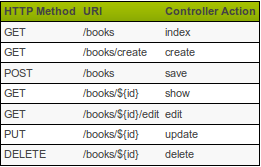
\includegraphics[width=5cm,height=3cm]{./images/DiagramaREST.png}
        \caption{Tabla de peticiones a Cute Bunny}
     \end{figure}
  \paragraph{Cute Bunny interactua con otros dos módulos de Ambienta2MX, Smart Owl y Hard Ant. La interacción con estos surge debido a que Hard Ant es el encargado de gestionar el acceso a las bases de datos de tipo MX y Smart Owl brindará y dará solución a las busquedas que no se encuentren en las bases de tipo MX, es decir, tratará de encontrar la información que Cute Bunny le solicitó para guardarla en algunas de las bases y posteriormente regresar el resultado al solicitante.}
      \begin{landscape}
        \subsubsection{Diagrama por bloques}
        \paragraph{A continuación se mostrará el diagrama por bloques que define la estructura de Cute Bunny.}
          \begin{figure}[b!]
          \centering
          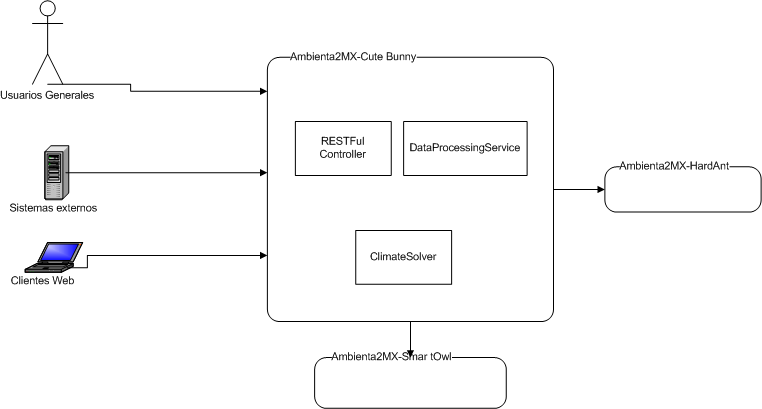
\includegraphics[width=22.5cm,height=12cm]{./images/DiagramaCuteBunny.png}
          \caption{Diagrama General de Cute Bunny}
        \end{figure}
      \end{landscape}